\section{Finite Element Method}

\begin{frame}
   \frametitle{Numerical methods for differential equations}

   \begin{figure}
    \centering
    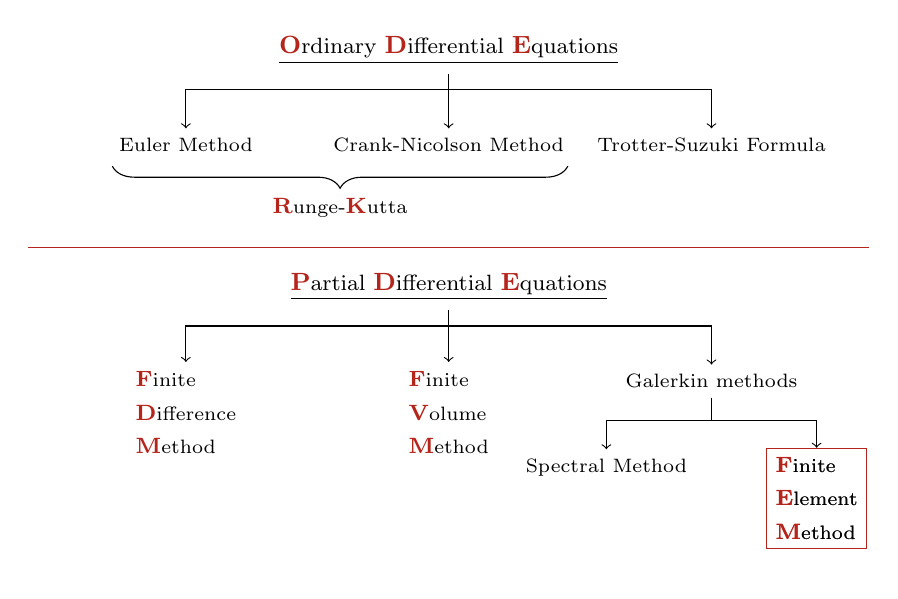
\begin{tikzpicture}[x=0.89cm]

        \node[align=left] at (0,5) (A) {\underline{\small{\textbf{\textcolor{BrickRed}{O}}}\footnotesize{rdinary }\small{\textbf{\textcolor{BrickRed}{D}}}\footnotesize{ifferential }\small{\textbf{\textcolor{BrickRed}{E}}}\footnotesize{quations}}};

        \node at (0,3.8) (B) {\scriptsize{Crank-Nicolson Method}};

        \node at (-3.75,3.8) (C) {\scriptsize{Euler Method}};

        \node at (3.75,3.8) (D) {\scriptsize{Trotter-Suzuki Formula}};

        \draw[->] (A) -- (B);
        \draw[->] (0,4.5) -- (-3.75,4.5) -- (C);
        \draw[->] (0,4.5) -- (3.75,4.5) -- (D);

        \draw[decorate, decoration={brace, amplitude=8pt, raise=2pt}] (1.7,3.6) -- (-4.8,3.6);
        \node at (-1.55,3) (E) {\footnotesize{\textbf{\textcolor{BrickRed}{R}}}\scriptsize{unge-}\footnotesize{\textbf{\textcolor{BrickRed}{K}}}\scriptsize{utta}};

         

        \draw[BrickRed] (-6,2.5) -- (6,2.5);



        \node[align=left] at (0,2) (F) {\underline{\small{\textbf{\textcolor{BrickRed}{P}}}\footnotesize{artial }\small{\textbf{\textcolor{BrickRed}{D}}}\footnotesize{ifferential }\small{\textbf{\textcolor{BrickRed}{E}}}\footnotesize{quations}}};

        \node[align=left] at (0,0.4) (G) {\footnotesize{\textbf{\textcolor{BrickRed}{F}}}\scriptsize{inite}\\\footnotesize{\textbf{\textcolor{BrickRed}{V}}}\scriptsize{olume}\\\footnotesize{\textbf{\textcolor{BrickRed}{M}}}\scriptsize{ethod}};

        \node[align=left] at (-3.75,0.4) (H) {\footnotesize{\textbf{\textcolor{BrickRed}{F}}}\scriptsize{inite}\\\footnotesize{\textbf{\textcolor{BrickRed}{D}}}\scriptsize{ifference}\\\footnotesize{\textbf{\textcolor{BrickRed}{M}}}\scriptsize{ethod}};

        \node at (3.75,0.8) (I) {\scriptsize{Galerkin methods}};

        \node at (2.25,-0.3) (J) {\scriptsize{Spectral Method}};

        \node<1>[align=left] at (5.25,-0.69) (Ktext) {\footnotesize{\textbf{\textcolor{BrickRed}{F}}}\scriptsize{\textcolor{black}{inite}}\\\footnotesize{\textbf{\textcolor{BrickRed}{E}}}\scriptsize{\textcolor{black}{lement}}\\\footnotesize{\textbf{\textcolor{BrickRed}{M}}}\scriptsize{\textcolor{black}{ethod}}};

        \node<2->[draw,BrickRed,align=left] at (5.25,-0.69) (K) {\footnotesize{\textbf{\textcolor{BrickRed}{F}}}\scriptsize{\textcolor{black}{inite}}\\\footnotesize{\textbf{\textcolor{BrickRed}{E}}}\scriptsize{\textcolor{black}{lement}}\\\footnotesize{\textbf{\textcolor{BrickRed}{M}}}\scriptsize{\textcolor{black}{ethod}}};

        \draw[->] (F) -- (G);
        \draw[->] (0,1.5) -- (-3.75,1.5) -- (H);
        \draw[->] (0,1.5) -- (3.75,1.5) -- (I);
        \draw[->] (I) -- (3.75,0.3) -- (2.25,0.3) -- (J);
        \draw[->] (I) -- (3.75,0.3) -- (5.25,0.3) -- (Ktext);



        \draw[white] (0,-1.6) -- (0,-1.5);
    \end{tikzpicture}
\end{figure}
\end{frame}

\begin{frame}{Introduction to the problem}
   Solving a \textbf{\textcolor{BrickRed}{PDE}} means to find a function $u$ such that

   \begin{equation*}
      \mathcal{L}u=f
   \end{equation*}

   where $\mathcal{L}$ is a \underline{differential operator} and $f$ is a \underline{source term}.

   \vspace{0.3cm}

   The equation holds in a domain $\Omega$ and is completed by prescribing \textbf{boundary conditions} on $\partial\Omega$.

   \vfill

   \pause

   \begin{figure}[H]
    \centering
    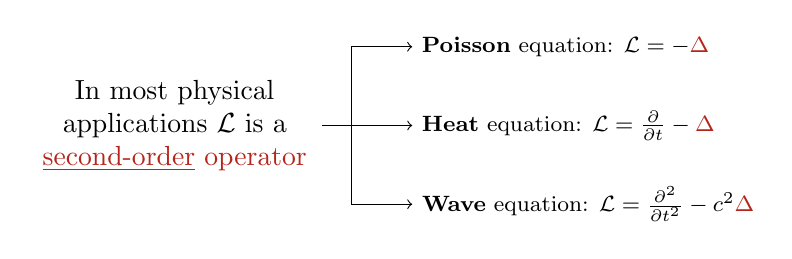
\begin{tikzpicture}
        \node[align=center,text width=3.5cm] at (0,0) (A) {In most physical applications $\mathcal{L}$ is a \textcolor{BrickRed}{\underline{second-order} operator}};

        \node at (5,0) (B) {\footnotesize{\textbf{Heat} equation: $\mathcal{L}=\frac{\partial}{\partial t}-\textcolor{BrickRed}{\Delta}$}};

        \node at (4.965,1) (C) {\footnotesize{\textbf{Poisson} equation: $\mathcal{L}=-\textcolor{BrickRed}{\Delta}$}};

        \node at (5.25,-1) (D) {\footnotesize{\textbf{Wave} equation: $\mathcal{L}=\frac{\partial^2}{\partial t^2}-c^2\textcolor{BrickRed}{\Delta}$}};

        \draw[->] (A) -- (B);
        \draw[->] (2.25,0) -- (2.25,1) -- (C);
        \draw[->] (2.25,0) -- (2.25,-1) -- (D); 
    \end{tikzpicture}
\end{figure}
\end{frame}

\subsection{Galerkin methods}

\begin{frame}{Weak formulation}
   Galerkin methods rely on a \textbf{\textcolor{BrickRed}{weak formulation}}

   \vspace{0.5cm}

   \pause

   \begin{itemize}
      \item \underline{Multiply} by a \textcolor{BrickRed}{test function} $v$ and \underline{integrate} over the entire domain
      
      \begin{equation*}
         -\int_\Omega(\Delta u)vd\Omega=\int_\Omega fvd\Omega
      \end{equation*}

      \pause

      \item \underline{Integrate by parts} the left hand side
      
      \begin{equation*}
         -\int_\Omega(\Delta u)vd\Omega=\int_\Omega\nabla u\cdot\nabla vd\Omega-\int_{\partial\Omega}\frac{\partial u}{\partial n}vds
      \end{equation*}

      \pause

      \item \underline{Substitute} and get the new expression
      
      \begin{equation*}
         \int_\Omega\nabla u\cdot\nabla vd\Omega=\int_\Omega fvd\Omega+\int_{\partial\Omega}\frac{\partial u}{\partial n}vds
      \end{equation*}
   \end{itemize}
\end{frame}

\begin{frame}{About the test function}
   \begin{center}
      \begin{framed}
         The test function $v$ is introduced to check whether the PDE is satisfied \textit{\underline{on average}} throughout the domain.
      \end{framed}
   \end{center}

   \pause

   The problem becomes to find $u$ such that

   \begin{equation*}
      a(u,v)=F(v) \qquad \forall v\in V
   \end{equation*}

   where

   \begin{alignat*}{2}
      a(u,v)&=\int_\Omega\nabla u\cdot\nabla vd\Omega \qquad &&\text{is a \underline{bilinear form}}\\
      F(v)&=\int_\Omega fvd\Omega+\int_{\partial\Omega}\frac{\partial u}{\partial n}vds \qquad &&\text{is a \underline{linear functional}}
   \end{alignat*}
\end{frame}

\begin{frame}{Benefits of the weak formulation}
   \begin{table}[H]
    \centering
    \begin{tabular}{c c}
        \textbf{Strong formulation} & \textbf{Weak formulation}\\
        \hline
        $u\in C^2(\Omega)$ & $u,v\in H^1(\Omega)^{\boldsymbol{\textcolor{BrickRed}{\ast}}}$\\
        Holds pointwise in $\Omega$ & Holds on average on $\Omega$\\
        Derivatives exist classically & \renewcommand{\arraystretch}{0.8} \begin{tabular}{@{}c@{}}Derivatives exist in the \\ distributional sense\end{tabular}\\
        \textcolor{white}{Derivatives exist classicallyyyy} & \textcolor{white}{Derivatives exist classicallyyyy}
    \end{tabular}
\end{table}

   \vspace{-0.5cm}

   \uncover<2->{\begin{center}
      \begin{framed}
         In short: weak formulation requires \textbf{\textcolor{BrickRed}{less regularity}}
      \end{framed}
   \end{center}}

   \vspace{0.6cm}

   $^{\boldsymbol{\textcolor{BrickRed}{\ast}}}$\scriptsize{$H^1(\Omega)$ is a \textbf{Sobolev space} of functions with square-integrable first derivatives:}

   \begin{equation*}
      w\in H^1(\Omega)=\left\{w\in L^2(\Omega)\mid\nabla w\in L^2(\Omega)^d\right\}
   \end{equation*}

   \normalsize
\end{frame}

\begin{frame}{On boundary conditions}
   Another difference lies in the boundary condition prescription.

   \vspace{0.35cm}

   \pause

   \begin{figure}[H]
    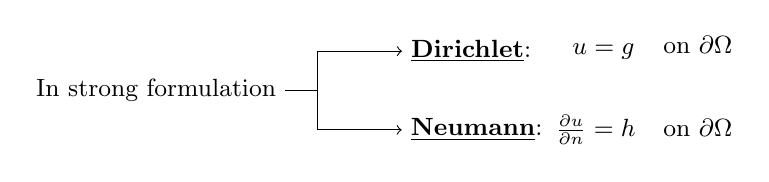
\begin{tikzpicture}

        \small

        \node at (0,0) (A) {In strong formulation};
        \node at (4,0.5) (B) {\underline{\textbf{Dirichlet}}:};
        \node at (4.07,-0.5) (C) {\underline{\textbf{Neumann}}:};

        \node at (5.68,0.5) () {$u=g$};
        \node at (5.58,-0.5) () {$\frac{\partial u}{\partial n}=h$};

        \node at (6.88,0.58) () {on $\partial\Omega$};
        \node at (6.88,-0.48) () {on $\partial\Omega$};

        \draw[->] (A) -- (2.05,0) -- (2.05,0.5) -- (B);
        \draw[->] (2.05,0) -- (2.05,-0.5) -- (C);

        \normalsize
    \end{tikzpicture}
\end{figure}

   \vspace{-0.5cm}

   \pause

   \begin{figure}[H]
    \centering
    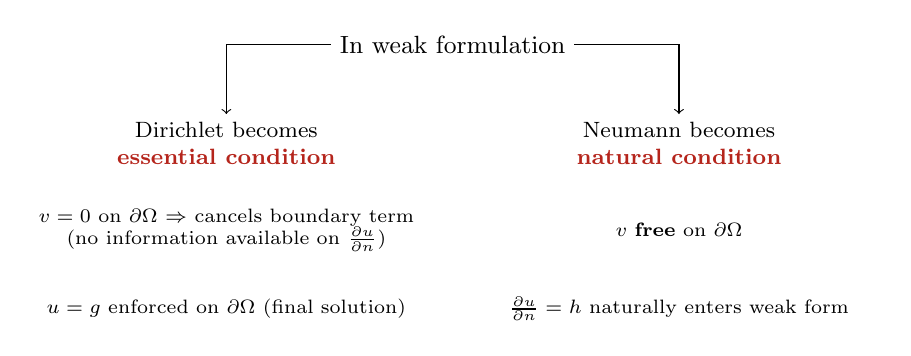
\begin{tikzpicture}
        \small

        \node at (0,5) (A) {In weak formulation};

        \footnotesize

        \node[align=center] at (-2.874,3.75) (B) {Dirichlet becomes\\ \textbf{\textcolor{BrickRed}{essential condition}}};
        \node[align=center] at (2.874,3.75) (C) {Neumann becomes\\ \textbf{\textcolor{BrickRed}{natural condition}}};

        \scriptsize

        \node[align=center,text width=4.86cm] at (-2.874,2.65) (D) {$\boldsymbol{v=0}$ on $\partial\Omega$ $\Rightarrow$ cancels boundary term\\ (no information available on $\frac{\partial u}{\partial n}$)};

        \node[align=center,text width=4.86cm] at (-2.874,1.65) (E) {$\boldsymbol{u=g}$ enforced on $\partial\Omega$ (final solution)};

        \node[align=center,text width=5cm] at (2.874,2.65) (F) {$\boldsymbol{v}$ \textbf{free} on $\partial\Omega$};

        \node[align=center,text width=5cm] at (2.874,1.65) (G) {$\boldsymbol{\frac{\partial u}{\partial n}=h}$ naturally enters weak form};

        \draw[->] (A) -- (-2.874,5) -- (B);
        \draw[->] (A) -- (2.874,5) -- (C);

        \normalsize
    \end{tikzpicture}
\end{figure}
\end{frame}

\begin{frame}{Shape functions}
   Galerkin methods allow to find an \underline{approximate solution}
   
   \begin{equation*}
      u_h\in V_h\subset H^1(\Omega) \qquad \text{where } V_h \ \text{is a \textbf{finite-dimensional} space} 
   \end{equation*}

   In this framework, the goal is to find $u_h$ such that

   \begin{equation*}
      \boxed{a\left(u_h,v_h\right)=F\left(v_h\right) \qquad \forall v_h\in V_h}
   \end{equation*}

   \vfill

   \pause

   A \textbf{basis of function} $\left\{\phi_i\right\}$ is chosen to express $u_h$ and to use it as \underline{test}:

   \begin{equation*}
      u_h=\sum_{j=1}^Nu_j\phi_j \ \Longrightarrow \ a\left(\sum_{j=1}^Nu_j\phi_j,\phi_i\right)=F\left(\phi_i\right) \qquad \forall i=1,\dots,N
   \end{equation*}

   \vfill

   \pause

   \begin{center}
      Functions $\phi_i$ model the solution $\longrightarrow$ \textbf{\textcolor{BrickRed}{shape functions}}
   \end{center}
\end{frame}

\begin{frame}{Final expression}
   By linearity of $a(\cdot,\cdot)$, the problem reduces to a \textbf{finite linear system}:

   \begin{equation*}
      \sum_{j=1}^Nu_ja\left(\phi_j,\phi_i\right)=F\left(\phi_i\right) \qquad \forall i=1,\dots,N
   \end{equation*}

   \vspace{-0.1cm}

   \begin{equation*}
      \Big\Downarrow
   \end{equation*}

   \vspace{-0.1cm}

   \begin{equation*}
      \fcolorbox{BrickRed}{white}{\text{$A\boldsymbol{u}=\boldsymbol{F}$}}
   \end{equation*}

   \pause

   where

   \begin{alignat*}{2}
      A_{i,j}&=a\left(\phi_j,\phi_i\right) &&\text{form the \textbf{\textcolor{BrickRed}{stiffness matrix}}}\\
      \boldsymbol{u}&=\left(u_1,\dots,u_N\right)^T &&\text{is the \textbf{\textcolor{BrickRed}{vector of unknowns}}}\\
      \boldsymbol{F}&=\left(F\left(\phi_1\right),\dots,F\left(\phi_N\right)\right)^T \qquad &&\text{is the \textbf{\textcolor{BrickRed}{load vector}}} 
   \end{alignat*}
\end{frame}

\subsection{Elements definition}

\begin{frame}{Mesh discretization}
   \begin{center}
      \begin{framed}
         \textbf{FEM} approach consists in the subdivision of the domain in a so-called \textbf{\textcolor{BrickRed}{mesh}}
      \end{framed}
   \end{center}

   \pause

   This choice brings several advantages:

   \begin{itemize}
      \item Good approximation of \textbf{complex geometries}
      \item Better capture of \textbf{local effects}
      \item Possibility of \textbf{adaptive refinement}
      \item Natural construction of a \textbf{global solution}
   \end{itemize}

   \visible<2>{\begin{figure}[H]
      \centering
      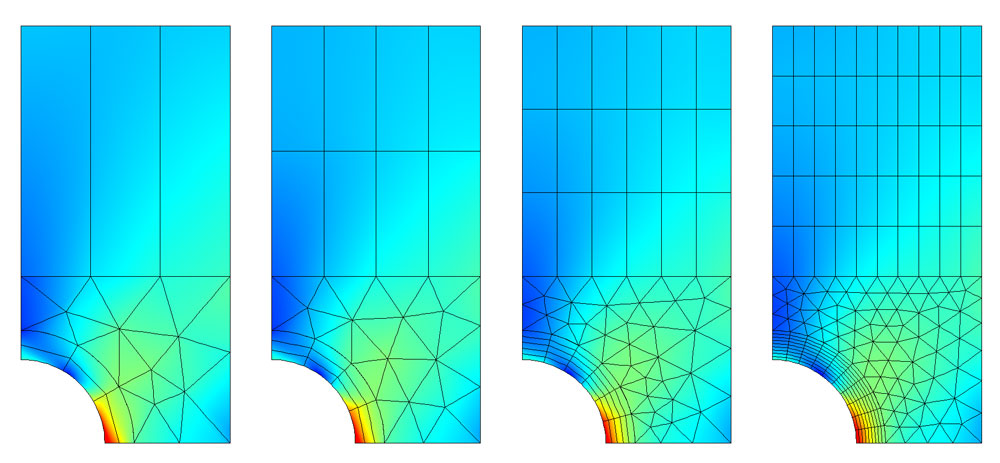
\includegraphics[width=0.68\textwidth]{Immagini/mesh-example.jpeg}
   \end{figure}}
\end{frame}

\begin{frame}{Elements}
   \begin{figure}[H]
    \centering
    \begin{tikzpicture}
        \scriptsize

        \node at (0,2) (A) {Discretization in different dimensions};
        \node at (-4,1.4) (B) {1D};
        \node at (0,1.4) (C) {2D};
        \node at (4,1.4) (D) {3D};

        \draw[->] (A) -- (C);
        \draw[->] (A) -- (-4,2) -- (B);
        \draw[->] (A) -- (4,2) -- (D);

        \node at (-4,0.7) (E) {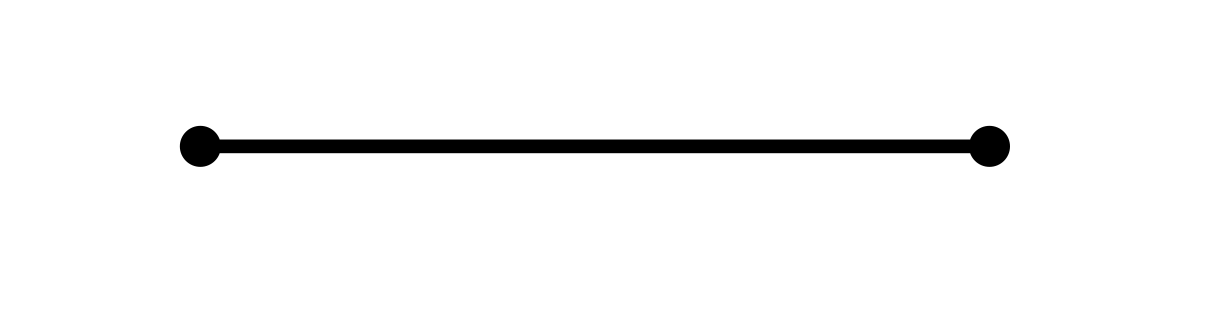
\includegraphics[width=0.218\textwidth]{Immagini/element-1D.png}};
        \node at (0,0.7) (F) {\includegraphics[width=0.2\textwidth]{Immagini/elements-2D.png}};
        \node at (4,0.68) (G) {\includegraphics[width=0.22\textwidth]{Immagini/elements-3D.png}};

        \visible<2->{\node at (-4,-1.8) (H) {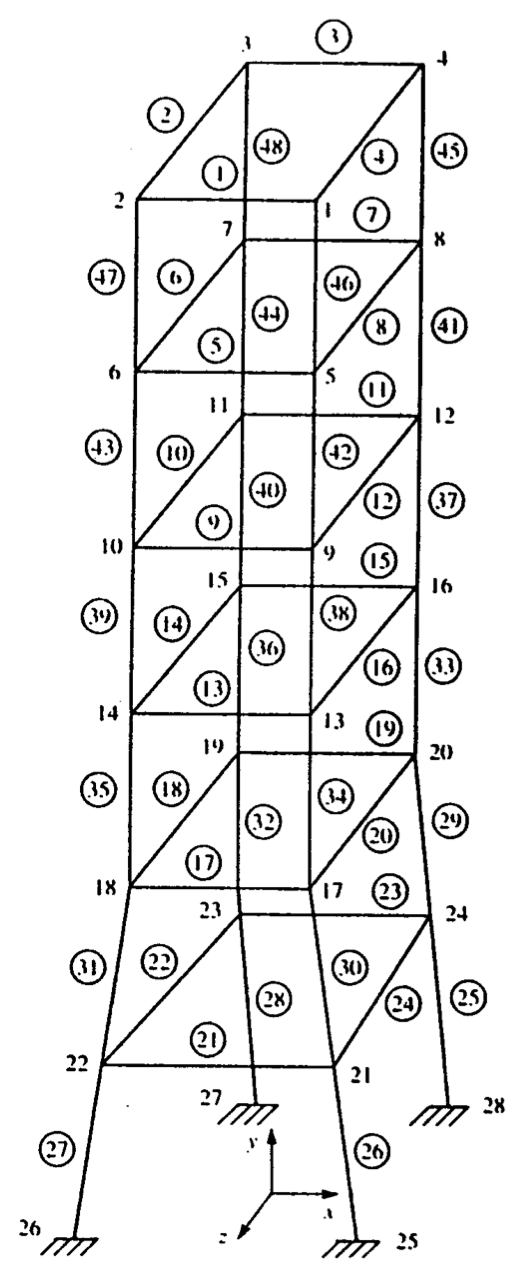
\includegraphics[width=0.14\textwidth]{Immagini/frame-elements.png}};
        \node at (-0.1,-1.9) (I) {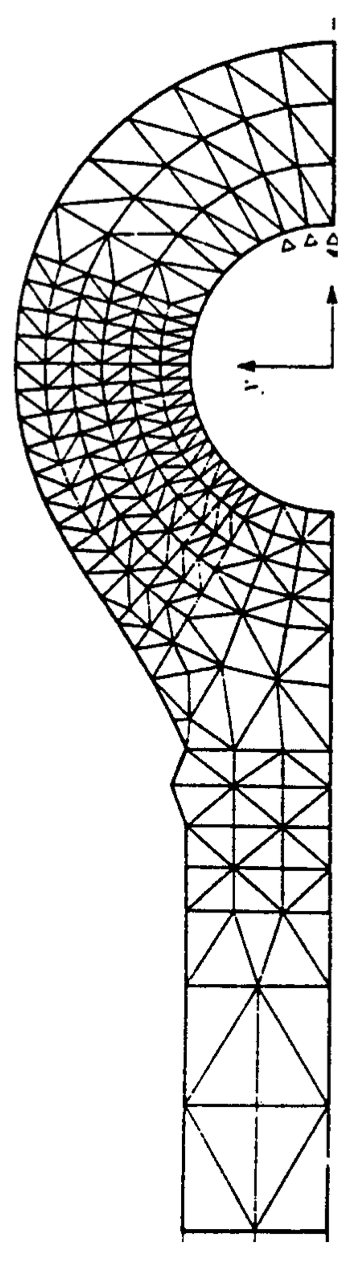
\includegraphics[width=0.1\textwidth]{Immagini/triangular elements.png}};
        \node at (3.78,-1.95) (J) {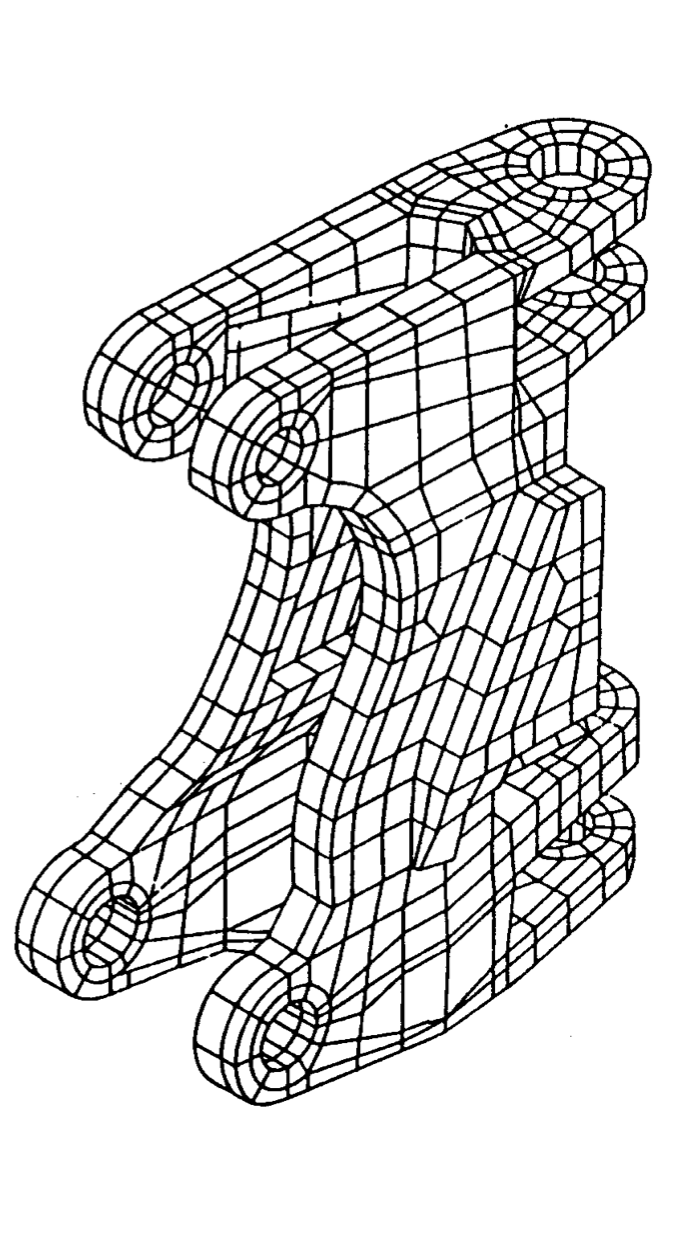
\includegraphics[width=0.21\textwidth]{Immagini/brick-elements.png}};

        \node at (-4,-4.1) (K) {\textbf{Frame \textcolor{BrickRed}{elements}}};
        \node at (0,-4.1) (L) {\textbf{Triangular \textcolor{BrickRed}{elements}}};
        \node at (4,-4.1) (M) {\textbf{Brick \textcolor{BrickRed}{elements}}};}

        \visible<3->{\draw[decorate, decoration={brace, amplitude=8pt, raise=2pt}] (5.25,-4.25) -- (-5.25,-4.25);

        \node at (0,-4.85) (N) {\textbf{Finite \textcolor{BrickRed}{Element} Method}};}

        \normalsize
    \end{tikzpicture}
\end{figure}
\end{frame}

\begin{frame}{Application examples}
   \begin{minipage}{0.5\textwidth}
      \begin{figure}[H]
         \raggedright
         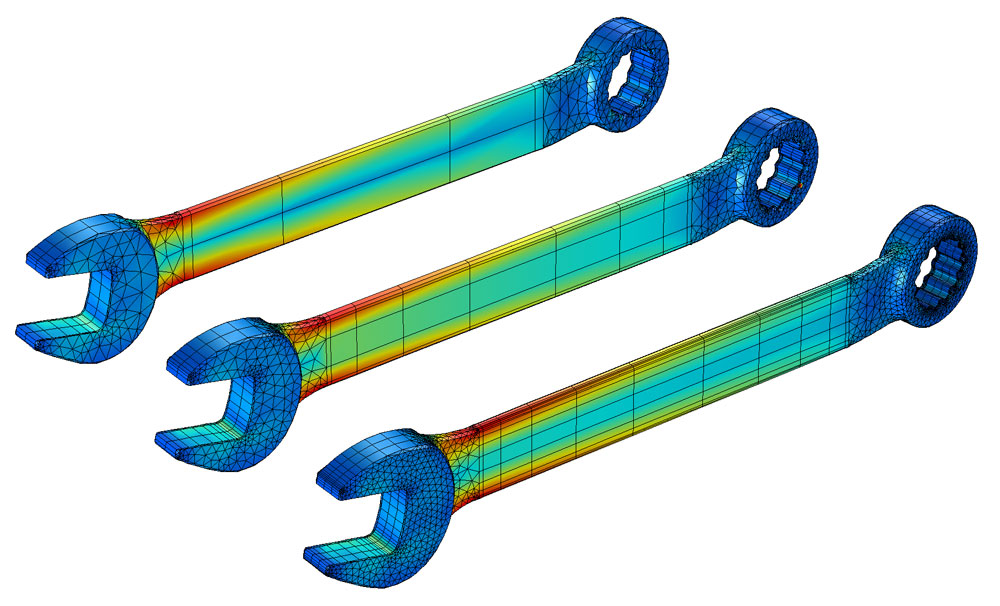
\includegraphics[width=\textwidth]{Immagini/mesh-application-1.jpeg}
      \end{figure}
   \end{minipage}
   \hfill
   \begin{minipage}{0.45\textwidth}
      \footnotesize{\textit{Manual mesh refinement of a wrench using different element types}}

      \textcolor{white}{some}

      \tiny{\texttt{Image from COMSOL Multiplysics Cyclopedia, ``Finite Element Mesh Refinement'', 21st of February 2017}}
   \end{minipage}

   \vfill

   \begin{minipage}{0.425\textwidth}
      \footnotesize{\textit{Mesh of a wheel rim composed of tetrahedrons in green, bricks in blue and prisms in pink}}

      \textcolor{white}{some}

      \tiny{\texttt{Image from COMSOL Multiplysics Blog, ``Meshing Your Geometry: When to Use the Various Element Types'', Walter Frei, 4th of November 2013}}
   \end{minipage}
   \hfill
   \begin{minipage}{0.5\textwidth}
      \begin{figure}[H]
         \raggedleft
         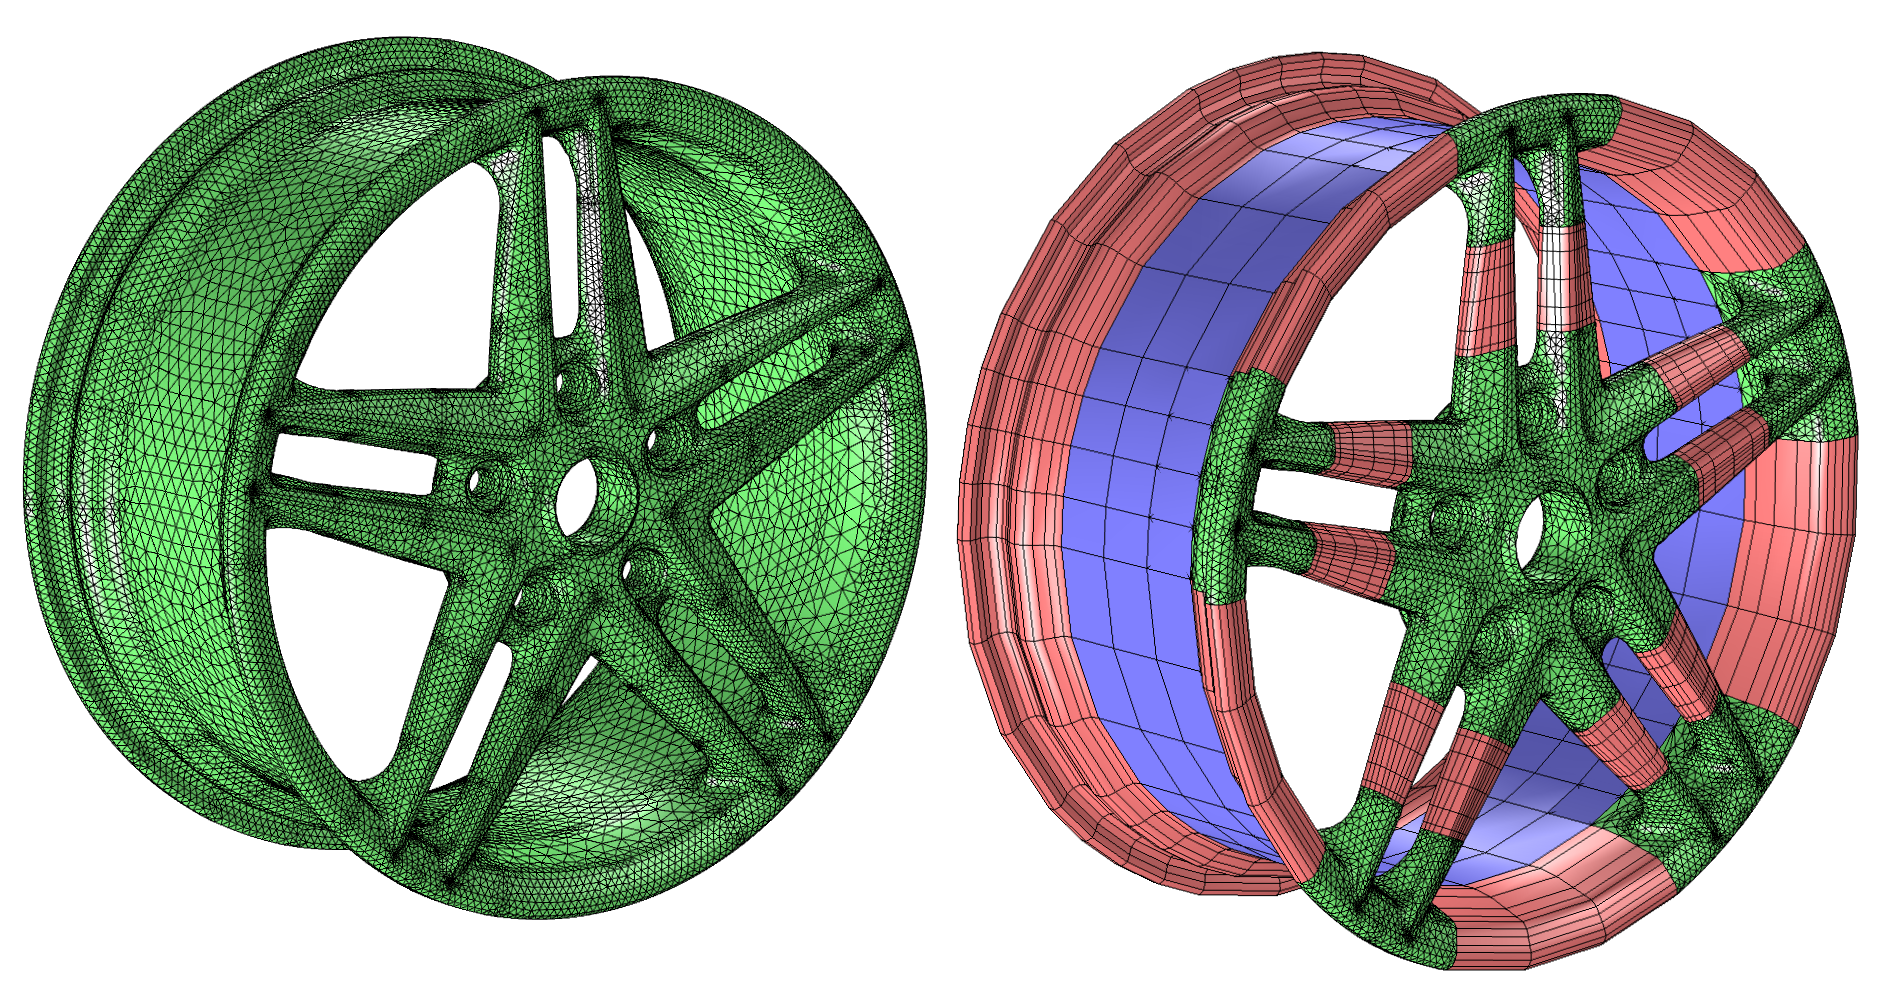
\includegraphics[width=\textwidth]{Immagini/mesh-application-2.png}
      \end{figure}
   \end{minipage}
\end{frame}

\begin{frame}{Choise of the base}
   \begin{figure}[H]
    \centering
    \begin{tikzpicture}
        \footnotesize

        \node at (0,2.4) (A) {Mesh division into sub-domains};

        \pause

        \draw[->] (0,2.05) -- (0,1.55);
        \node at (0,1.2) (B) {Choice of a \textbf{\textcolor{BrickRed}{local basis functions}}};

        \pause

        \draw[->] (0,0.85) -- (0,0.35);
        \node at (0,0) (C) {Exploitation of \underline{\textbf{compact support}}};

        \scriptsize

        \pause

        \node at (-3.458,-1.5) (D) {\textcolor{BrickRed}{$\bullet$} Leads to \textbf{sparse matrices}};
        \node at (-3.376,-2.25) (E) {\textcolor{BrickRed}{$\bullet$} Allows \textbf{local interpolation}};
        \node at (-3.174,-3) (F) {\textcolor{BrickRed}{$\bullet$} Enhances \textbf{numerical stability}};
        \node at (-3,-3.75) (G) {\textcolor{BrickRed}{$\bullet$} Enables \textbf{efficient parallelization}};

        \draw[->] (C) -- (-3.458,0) -- (D);

        \visible<4->{\node at (2.795,-2.58) (H) {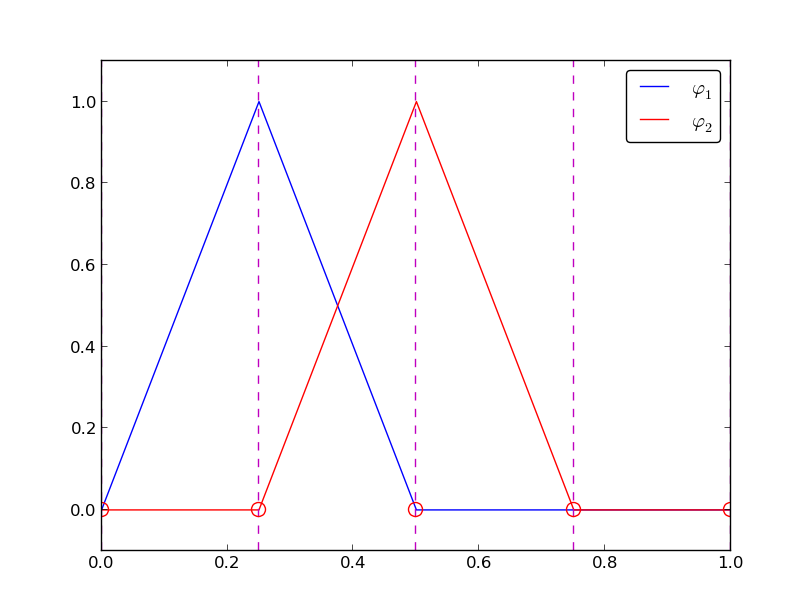
\includegraphics[width=0.45\textwidth]{Immagini/local-basis-functions.png}};}

        \normalsize
    \end{tikzpicture}
\end{figure}
\end{frame}

\subsection{Introduction to FEniCS}

\begin{frame}{FEniCS library}
   \small{A leading software platform for finite element computations is \textbf{\textcolor{BrickRed}{FEniCS}}.}

   \vfill

   \pause

   \scriptsize

   \begin{minipage}{0.38\textwidth}
      \begin{itemize}
         \item \textbf{Open-source} and freely available
         \item \textbf{Multi-language support} (\texttt{C++} and \texttt{Python} APIs)
         \item \textbf{Parallel computing} with MPI support
      \end{itemize}
   \end{minipage}
   \hfill
   \visible<2->{\begin{minipage}{0.57\textwidth}
      \begin{figure}[H]
         \centering
         
\includegraphics[width=\textwidth]{Immagini/fenics-logo.png}
      \end{figure}
   \end{minipage}}

   \vfill

   \pause

   \small

   \begin{equation*}
      \text{\texttt{FEniCS} package:}
      \begin{cases}
         \text{\texttt{DOLFIN}} \ &\text{(backend core engine and \texttt{PETSc} interface)}\\
         \text{\texttt{UFL}} \ &\text{(symbolic language)}\\
         \text{\texttt{FIAT}} \ &\text{(shape functions tabulator)}\\
         \text{\texttt{FFC}} \ &\text{(\texttt{C++} compiler for efficient local assembly)}\\
         \text{\texttt{MSHR}} \ &\text{(mesh generator)}
      \end{cases}
   \end{equation*}

   \normalsize
\end{frame}

\begin{frame}{A minimal FEniCS example: setup}
   \small{Setup of a \underline{Poisson equation} with Neumann boundary conditions in \texttt{FEniCS}:}

   \vspace{0.2cm}

   \begin{itemize}
      \item \small{Generation of the mesh}
      
      \begin{tcolorbox}[pythoncode]
         \footnotesize{\texttt{\textcolor{cyan!60!black}{domain} = \textcolor{violet!80!black}{mesh}.\textcolor{green!40!black}{create\_interval}(\textcolor{violet!80!black}{MPI}.\textcolor{green!40!black}{COMM\_WORLD}, \textcolor{cyan!60!black}{nx}, [\textcolor{brown!70!black}{0.0}, \textcolor{cyan!60!black}{L}])}}
      \end{tcolorbox}

      \item \small{Definition of the finite element function space}
      
      \begin{tcolorbox}[pythoncode]
         \footnotesize{\texttt{\textcolor{cyan!60!black}{V} = \textcolor{green!40!black}{functionspace}(\textcolor{cyan!60!black}{domain}, (\textcolor{red!80!black}{"Lagrange"}, \textcolor{brown!70!black}{1}))}}
      \end{tcolorbox}

      \item \small{Definition of trial function and test function}
      
      \begin{tcolorbox}[pythoncode]
         \footnotesize{\texttt{\textcolor{cyan!60!black}{u} = \textcolor{violet!80!black}{ufl}.\textcolor{green!40!black}{TrialFunction}(\textcolor{cyan!60!black}{V})}}

         \footnotesize{\texttt{\textcolor{cyan!60!black}{v} = \textcolor{violet!80!black}{ufl}.\textcolor{green!40!black}{TestFunction}(\textcolor{cyan!60!black}{V})}}
      \end{tcolorbox}

      \item \small{Definition of the source term}
      
      \begin{tcolorbox}[pythoncode]
         \footnotesize{\texttt{\textcolor{cyan!60!black}{f} = \textcolor{violet!80!black}{fem}.\textcolor{green!40!black}{Constant}(\textcolor{cyan!60!black}{domain}, \textcolor{green!40!black}{default\_scalar\_type}(\textcolor{brown!70!black}{-6}))}}
      \end{tcolorbox}
   \end{itemize}
\end{frame}

\begin{frame}{A minimal FEniCS example: solution}
   \small{Solving \underline{Poisson equation} with Neumann boundary conditions in \texttt{FEniCS}:}

   \vspace{0.2cm}

   \begin{itemize}
      \item \small{Weak formulation}
      
      \begin{tcolorbox}[pythoncode]
         \footnotesize{\texttt{\textcolor{cyan!60!black}{a} = \textcolor{violet!80!black}{ufl}.\textcolor{green!40!black}{dot}(\textcolor{violet!80!black}{ufl}.\textcolor{green!40!black}{grad}(\textcolor{cyan!60!black}{u}), \textcolor{violet!80!black}{ufl}.\textcolor{green!40!black}{grad}(\textcolor{cyan!60!black}{v})) * \textcolor{violet!80!black}{ufl}.\textcolor{green!40!black}{dx}}}

         \footnotesize{\texttt{\textcolor{cyan!60!black}{F} = \textcolor{cyan!60!black}{f} * \textcolor{cyan!60!black}{v} * \textcolor{violet!80!black}{ufl}.\textcolor{green!40!black}{dx}}}
      \end{tcolorbox}

      \item \small{Solution of the linear system}
      
      \begin{tcolorbox}[pythoncode]
         \footnotesize{\texttt{\textcolor{cyan!60!black}{problem} = \textcolor{green!40!black}{LinearProblem}(\textcolor{cyan!60!black}{a}, \textcolor{cyan!60!black}{F},}}
         
         \footnotesize{\texttt{\textcolor{gray!10}{aaaaaaaaaaaaaaaaaaaaaaaa}\textcolor{cyan!60!black}{petsc\_option} = \{\textcolor{red!80!black}{"ksp\_type"}: \textcolor{red!80!black}{"preonly"},}}
         
         \footnotesize{\texttt{\textcolor{gray!10}{aaaaaaaaaaaaaaaaaaaaaaaaaaaaaaaaaaaaaaaa}\textcolor{red!80!black}{"pc\_type"} : \textcolor{red!80!black}{"lu"}}}
         
         \footnotesize{\texttt{\textcolor{gray!10}{aaaaaaaaaaaaaaaaaaaaaaaaaaaaaaaaaaaaaa} \}}}
         
         \footnotesize{\texttt{\textcolor{gray!10}{aaaaaaaaaaaaaaaaaaaaaaa})}}

         \footnotesize{\texttt{\textcolor{cyan!60!black}{u\_h} = \textcolor{cyan!60!black}{problem}.\textcolor{green!40!black}{solve}()}}
      \end{tcolorbox}
   \end{itemize}

   \vfill
\end{frame}